% Tipo di documento. L'uso di twoside implica che i capitoli inizino sempre con la prima pagina a sinistra, eventualmente lasciando una pagina vuota nel capitolo precedente. Se questa cosa è fastidiosa, è possibile rimuoverlo. 
\documentclass[a4paper, openright]{report}

% Dimensione dei margini
\usepackage[a4paper,top=2cm,bottom=2cm,left=2cm,right=2cm]{geometry} 
% Dimensione del font
\usepackage[fontsize=12pt]{scrextend}
% Lingua del testo
\usepackage[english]{babel}
% Lingua per la bibliografia
\usepackage[fixlanguage]{babelbib}
% Codifica del testo
\usepackage[utf8]{inputenc} 
% Encoding del testo
\usepackage[T1]{fontenc}
% Per ruotare le immagini
\usepackage{rotating}
% Per modificare l'header delle pagine 
\usepackage{fancyhdr}               

% Librerie matematiche
\usepackage{amssymb}
\usepackage{amsmath}
\usepackage{amsthm}         

% Uso delle immagini
\usepackage{graphicx}
% Uso dei colori
\usepackage[dvipsnames]{xcolor}         
% Uso dei listing per il codice
\usepackage{listings}          
% Per inserire gli hyperlinks tra i vari elementi del testo 
\usepackage{hyperref}     
% Diversi tipi di sottolineature
\usepackage[normalem]{ulem}


\usepackage{blindtext}
\usepackage{titlesec}
\usepackage{ragged2e}
\usepackage{import}
\graphicspath{{./../../../}}

\definecolor{delim}{RGB}{20,105,176}
\definecolor{numb}{RGB}{106, 109, 32}
\definecolor{string}{rgb}{0.64,0.08,0.08}

\lstdefinelanguage{json}{
    numbers=left,
    numberstyle=\small,
    frame=single,
    rulecolor=\color{black},
    showspaces=false,
    showtabs=false,
    breaklines=true,
    postbreak=\raisebox{0ex}[0ex][0ex]{\ensuremath{\color{gray}\hookrightarrow\space}},
    breakatwhitespace=true,
    basicstyle=\ttfamily\small,
    upquote=true,
    morestring=[b]",
    stringstyle=\color{string},
    literate=
     *{0}{{{\color{numb}0}}}{1}
      {1}{{{\color{numb}1}}}{1}
      {2}{{{\color{numb}2}}}{1}
      {3}{{{\color{numb}3}}}{1}
      {4}{{{\color{numb}4}}}{1}
      {5}{{{\color{numb}5}}}{1}
      {6}{{{\color{numb}6}}}{1}
      {7}{{{\color{numb}7}}}{1}
      {8}{{{\color{numb}8}}}{1}
      {9}{{{\color{numb}9}}}{1}
      {\{}{{{\color{delim}{\{}}}}{1}
      {\}}{{{\color{delim}{\}}}}}{1}
      {[}{{{\color{delim}{[}}}}{1}
      {]}{{{\color{delim}{]}}}}{1},
}
\usepackage{xr}
\externaldocument{./appendix}
\newcommand{\cref}[1]{(Appendix \ref{#1})}


% Stile del codice
\lstdefinestyle{codeStyle}{
    % Colore dei commenti
    commentstyle=\color{teal},
    % Colore delle keyword
    keywordstyle=\color{Magenta},
    % Stile dei numeri di riga
    numberstyle=\tiny\color{gray},
    % Colore delle stringhe
    stringstyle=\color{violet},
    % Dimensione e stile del testo
    basicstyle=\ttfamily\footnotesize,
    % newline solo ai whitespaces
    breakatwhitespace=false,     
    % newline si/no
    breaklines=true,                 
    % Posizione della caption, top/bottom 
    captionpos=b,                    
    % Mantiene gli spazi nel codice, utile per l'indentazione
    keepspaces=true,                 
    % Dove visualizzare i numeri di linea
    numbers=left,                    
    % Distanza tra i numeri di linea
    numbersep=5pt,                  
    % Mostra gli spazi bianchi o meno
    showspaces=false,                
    % Mostra gli spazi bianchi nelle stringhe
    showstringspaces=false,
    % Mostra i tab
    showtabs=false,
    % Dimensione dei tab
    tabsize=2
} \lstset{style=codeStyle}


\newcounter{alphasect}
\def\alphainsection{0}

\let\oldsection=\section
\def\section{%
  \ifnum\alphainsection=1%
    \addtocounter{alphasect}{1}
  \fi%
\oldsection}%

\renewcommand\thesection{%
  \ifnum\alphainsection=1% 
    \Alph{alphasect}
  \else%
    \arabic{section}
  \fi%
}%

\newenvironment{alphasection}{%
  \ifnum\alphainsection=1%
    \errhelp={Let other blocks end at the beginning of the next block.}
    \errmessage{Nested Alpha section not allowed}
  \fi%
  \setcounter{alphasect}{0}
  \def\alphainsection{1}
}{%
  \setcounter{alphasect}{0}
  \def\alphainsection{0}
}



% Taken from Lena Herrmann at 
% http://lenaherrmann.net/2010/05/20/javascript-syntax-highlighting-in-the-latex-listings-package
\lstdefinelanguage{JavaScript}{
  keywords={typeof, new, true, false, catch, function, return, null, catch, switch, var, if, in, while, do, else, case, break},
  keywordstyle=\color{blue}\bfseries,
  ndkeywords={class, export, boolean, throw, implements, import, this},
  ndkeywordstyle=\color{darkgray}\bfseries,
  identifierstyle=\color{black},
  sensitive=false,
  comment=[l]{//},
  morecomment=[s]{/*}{*/},
  commentstyle=\color{purple}\ttfamily,
  stringstyle=\color{red}\ttfamily,
  morestring=[b]',
  morestring=[b]"
}

\lstset{
   language=JavaScript,
   backgroundcolor=\color{lightgray},
   extendedchars=true,
   basicstyle=\footnotesize\ttfamily,
   showstringspaces=false,
   showspaces=false,
   numbers=left,
   numberstyle=\footnotesize,
   numbersep=9pt,
   tabsize=2,
   breaklines=true,
   showtabs=false,
   captionpos=b
}


\begin{document}
\chapter{Graph database}
\justifying
The DBSM chosen for the graph database is Neo4j, it was use to manege the social part of the site and also to keep track of the reviews made for the feed and suggestion functionality.


The entities used in the database are:
\begin{itemize}
	\item User
	\item TopCritic
	\item Movie
\end{itemize}
The nodes themselves do not store a lot of data, we decided to keep the bare minimum by having the following attributes:
\begin{itemize}
	\item for the User and TopCritic:
	\begin{itemize}
		\item id
		\item name
	\end{itemize}
	\item for Movie:
	\begin{itemize}
		\item id
		\item title
	\end{itemize}
\end{itemize}
The relationship present are:
\begin{itemize}
	\item User -[:FOLLOWS]-> TopCritic
	\item User -[:REVIEWED]-> Movie
	\item TopCritic -[:REVIEWED]-> Movie
\end{itemize}
In particular the \emph{REVIEWED} relationship contains the following information:
\begin{itemize}
	\item content
	\item date
	\item freshness
\end{itemize}

Below is present a snapshot of the graph database taken from Neo4j.

\begin{figure}[H]
\begin{center}
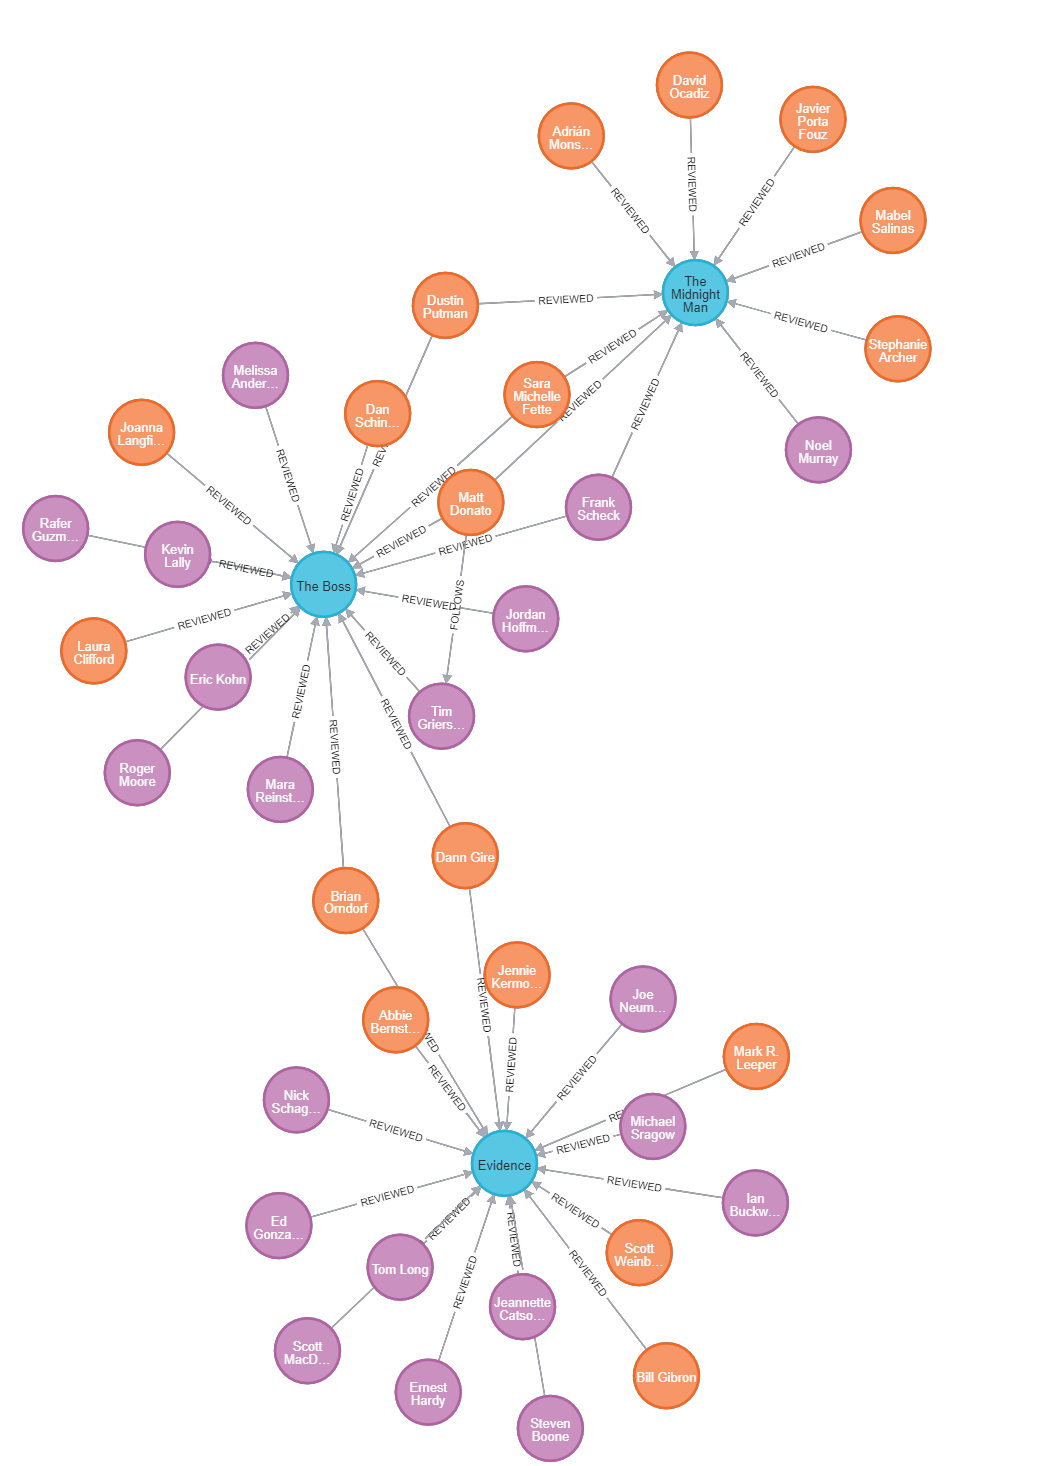
\includegraphics[scale=0.45]{/images/PNG/graph.png}
\caption{graph DB}
\label{fig:graphDB}
\end{center}
\end{figure}

As previously stated in the Feasibility study section \ref{sec:result}, the graph database design was heavily influenced by the document one, it was in fact generated by python script \cref{subsec:createGraphDB} that starts from the movie collection and, after generating the nodes for the \emph{Movie} entity, does the same for the user by dividing them between normal user and top critic. It then generates the \emph{REVIEWED} relationship based upon the data stored in the document database and finally it generates the \emph{FOLLOWS} relationship randomly

\section{Index}
The \emph{id} attributes is common to all nodes and it stores a string which is also used as id by the document database in the \emph{\textunderscore id} field, this choice was made so that we could have a way to identify the same object across the different databases with only one string from the application. Due to the OOP language used to build the latter the data was manipulated with classes containing the id of the object so, to improved the performance of the graph database we decided to use the \emph{id} attribute as a index. 

Below the information in a json format from the Neo4j DBSM about the new index (some attributes were omitted for space)
\lstinputlisting[language=json]{./../code/graphIndex.json}

We then proceed to confront the profile of the queries with and without the above indexes, here we can see the result of this analysis: 
\begin{figure}[H]
\begin{center}
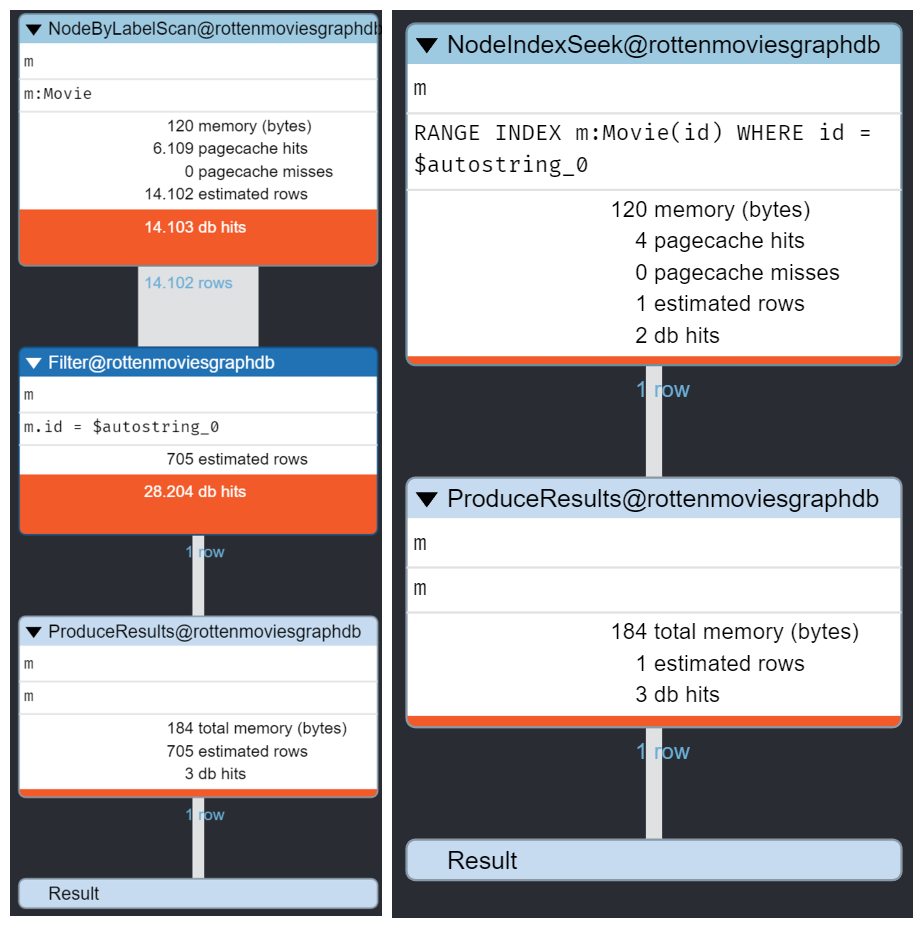
\includegraphics[scale=0.33]{/images/neo4j_stats/find_movie_by_id.png}
\caption{search by id without and with movie\textunderscore id \textunderscore index}
\label{fig:movieId}
\end{center}
\end{figure}

\begin{figure}[H]
\begin{center}
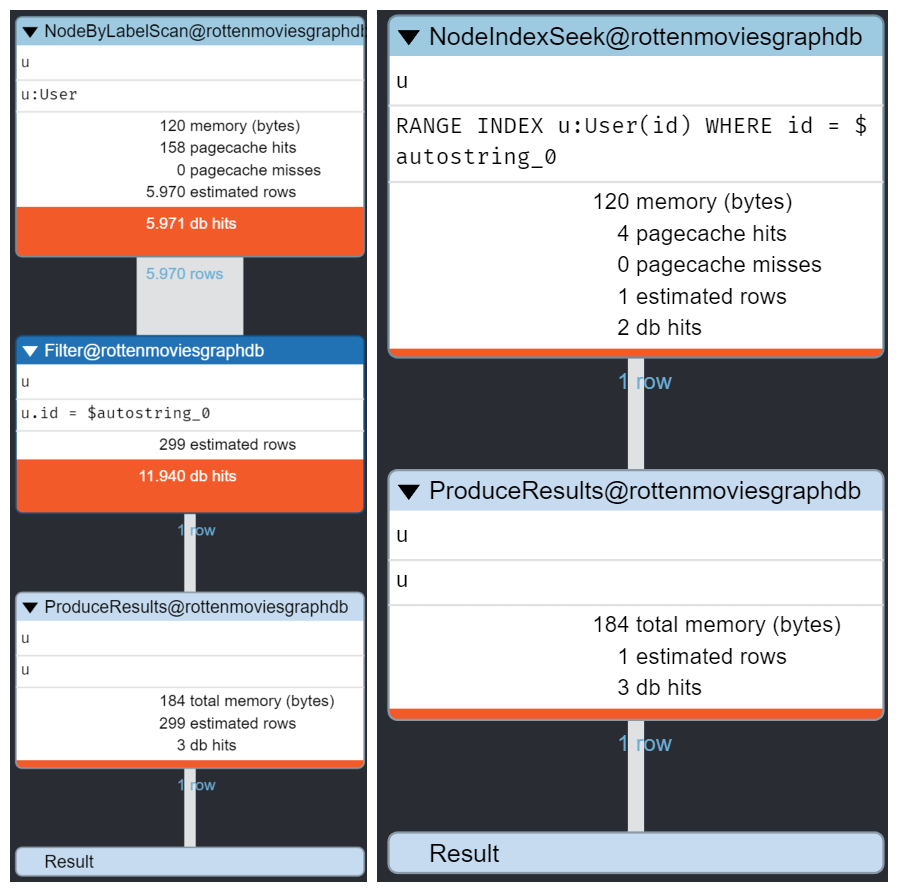
\includegraphics[scale=0.33]{/images/neo4j_stats/find_user_by_id.png}
\caption{search by id without and with user\textunderscore id \textunderscore index}
\label{fig:userId}
\end{center}
\end{figure}


\section{Queries}
In the following section we will show the queries that drove the design of the graph database.
\begin{center}
\begin{tabular}{|p{8cm} ||p{8cm}|}
\hline
Graph-Centric Query & Domain-Specific Query \\
\hline\hline
Which are the User nodes with the most outgoing edges of type REVIEWED & Which are the non top critic user with most reviews made\\
\hline
Which are the TopCritic nodes with the most incoming edges of type FOLLOWS & Which are the most followed top critics \\
\hline
Which are the Movies nodes that have been most recently connected with TopCritic nodes by a REVIEWED relationship meanwhile the latter are connected to a User node with a FOLLOWS relationship & Which are the latest reviewed movies by a followed top critics given a starting user \\
\hline
Which are the User and TopCritic nodes that have outgoing REVIEWED edges to the same Movie node without having a FOLLOWS edge between them, which of these TopCritic nodes have more similar attribute on the REVIEWED relationship with the one on the same type going towards the same Movie node given a User node & Which are the non-followed top critics with the most affinity towards a given user\\
\hline
Which Movie nodes have different ratio of freshness in the incoming REVIEWED edges spitted in base of their date attribute & Which movies have been targeted by review bombing in the last x month\\
\hline
\end{tabular}
\end{center}
\end{document}